\documentclass{article}
\usepackage{amsmath,amssymb, amsfonts}
\usepackage{algorithm}
\usepackage{float}
\usepackage{subcaption}
 \usepackage{relsize}
\usepackage{graphicx}
\usepackage{booktabs} 
\usepackage[table]{xcolor}
\usepackage{bm}
\usepackage{setspace}
\usepackage{amsthm}
\usepackage{graphicx}
\usepackage{algorithm}
\usepackage{algpseudocode}
\usepackage{cite}
\usepackage{geometry}
 \geometry{
 letterpaper,
 total={8.5in,11in},
 left=1.25in,
 right=1in,
 top=1in,
 bottom=1in,
 }
\doublespace

\newcommand{\commJoey}[1]{{\color{red}{\em Joey: #1}}}
\newcommand{\commTim}[1]{{\color{blue}{\em Tim: #1}}}
\newcommand{\commPierre}[1]{{\color{green}{\em Pierre: #1}}}

\def\r{{\mathbb R}}

\begin{document}
All of the work described below uses the model Tim emailed to Joey on October 13, 2017; the codes are included in OO-NVU-20.zip saved in the repository. Our objective is to identify which parameters in the model govern the dynamics of the potassium, the state $K_e$ in the model, during the period when a current is applied.

As a first step we allowed 70 parameters to vary on a uniform interval about their nominal value with 10\% uncertainty. These 70 parameters are found in the following channels within the ``Neuron.m" file contained in OO-NVU-20.zip,
\begin{enumerate}
\item[$\bullet$] Na flux through NaP channel in soma using GHK
\item[$\bullet$] Na flux through NaT channel in soma using GHK
\item[$\bullet$] K flux through KDR channel in soma using GHK
\item[$\bullet$] K flux through KA channel in soma using GHKinput\_current
\item[$\bullet$] Na flux through NaP channel in dendrite using GHK
\item[$\bullet$] Na/K flux through NMDA channel in dendrite using GHK
\item[$\bullet$] K flux through KDR channel in dendrite using GHK
\item[$\bullet$] K flux through KA channel in dendrite using GHK
\end{enumerate}

We generated 1000 realizations of these parameters (assuming them to be independent) and solved the ODE system for each realization. Of these 1000 realizations, 167 of them did not return a solution for the entire time interval; we expect that the ODE solver was unable to solve for those parameter values. There were also 3 realizations where the ODE solver returned complex solutions, these where discarded as well. This left 830 realizations to be used for the subsequent analysis.

Using the 830 realizations we are able to identify that around 24 of them yielded a potassium profile consistent with experimental data. This seems to indicate that there exists a subset of the parameters under consideration which give the desired dynamics. Upon inspection of histograms and correlation plots, we hypothesize that to understand the parameters yielding results comparable to experimental data we must understand the correlation structure of the parameters. We assumed them to be independent because we have no further knowledge at this time. If we can solve a Bayesian inverse problem we may discovered the desired correlation structure, but this is too computationally intensive with the current parameter dimension and model complexity. 

Using the 830 realizations we constructed a KL expansion of the process and learned the coefficient functions with a radial basis functions model. This gave a surrogate model from which we computed the total Sobol' indices, they are plotted in Figure~\ref{fig:all_parameters}.

Because of the high parameter dimension there are possible surrogate approximation errors which could alter the Sobol' indices. To reduce the dimension we did analysis on each channel so that through a collection of lower dimensional problems we may compute Sobol' indices and extract important parameters from each channel. In this analysis we included four additional parameters in the buffer equation, search ``change in buffer for K+ in the extracellular space" in Neuron.m to find this equation. This is a total of 74 parameters partitioned over 8 channels and a buffer in the model. Figure~\ref{fig:channelwise_variances} shows the time dependent variance of $K_e$ as parameters are varied within each channel. We have omitted the buffer parameters experiment from this plot as it had negligible variance. The results of Figure~\ref{fig:channelwise_variances} are consistent with Figure~\ref{fig:all_parameters}. There are three channel in Figure~\ref{fig:channelwise_variances} which are nearly 0 so we no longer consider varying those parameters. For each of the 5 channels with nontrivial variance, we constructed surrogate models as we did for the full 70 parameter model and computed total Sobol' indices. The results are shown in Figure~\ref{fig:channelwise_sobol}. These results are consistent with what we observed when varying all 70 parameters. Hence by analyzing them one channel at a time we simplify the construction of surrogate models and computation of Sobol' indices, but the results agree with the case were we vary all 70 parameters. This validates that Figure~\ref{fig:all_parameters} is a trustworthy assessment of the parameters influence.

\newpage
\begin{figure}[h]
\begin{center}
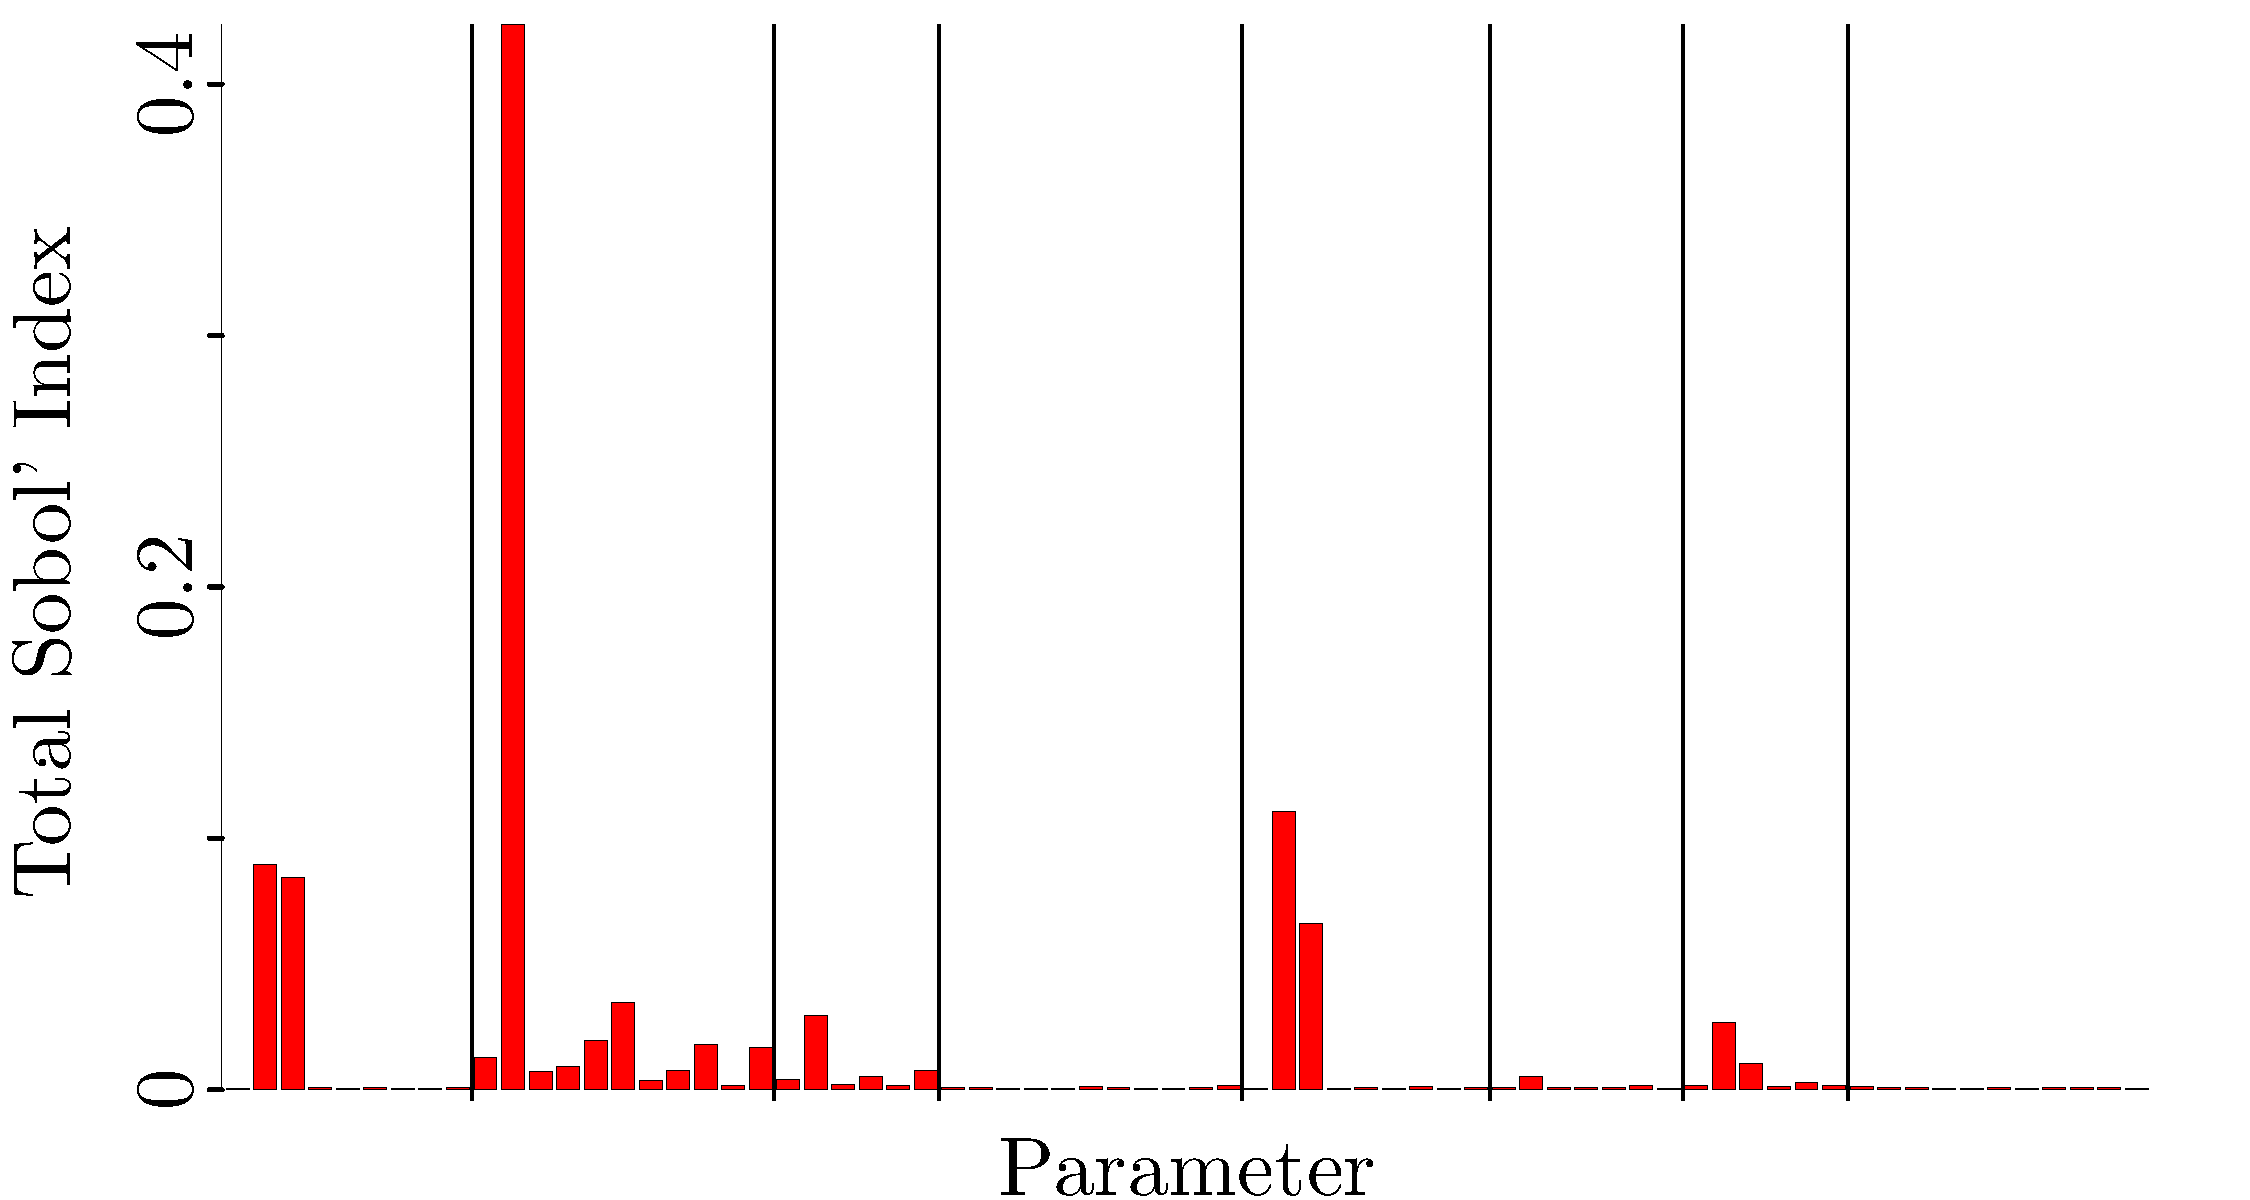
\includegraphics[scale=.25]{Figures/All_Parameters.pdf}
\end{center}
\caption{Total Sobol' indices for 70 parameters in the 8 channels. The black vertical lines are separating the channels. There are 13 parameters whose total Sobol' index is greater than 0.01.}
\label{fig:all_parameters}
\end{figure}

\begin{figure}[h]
\begin{center}
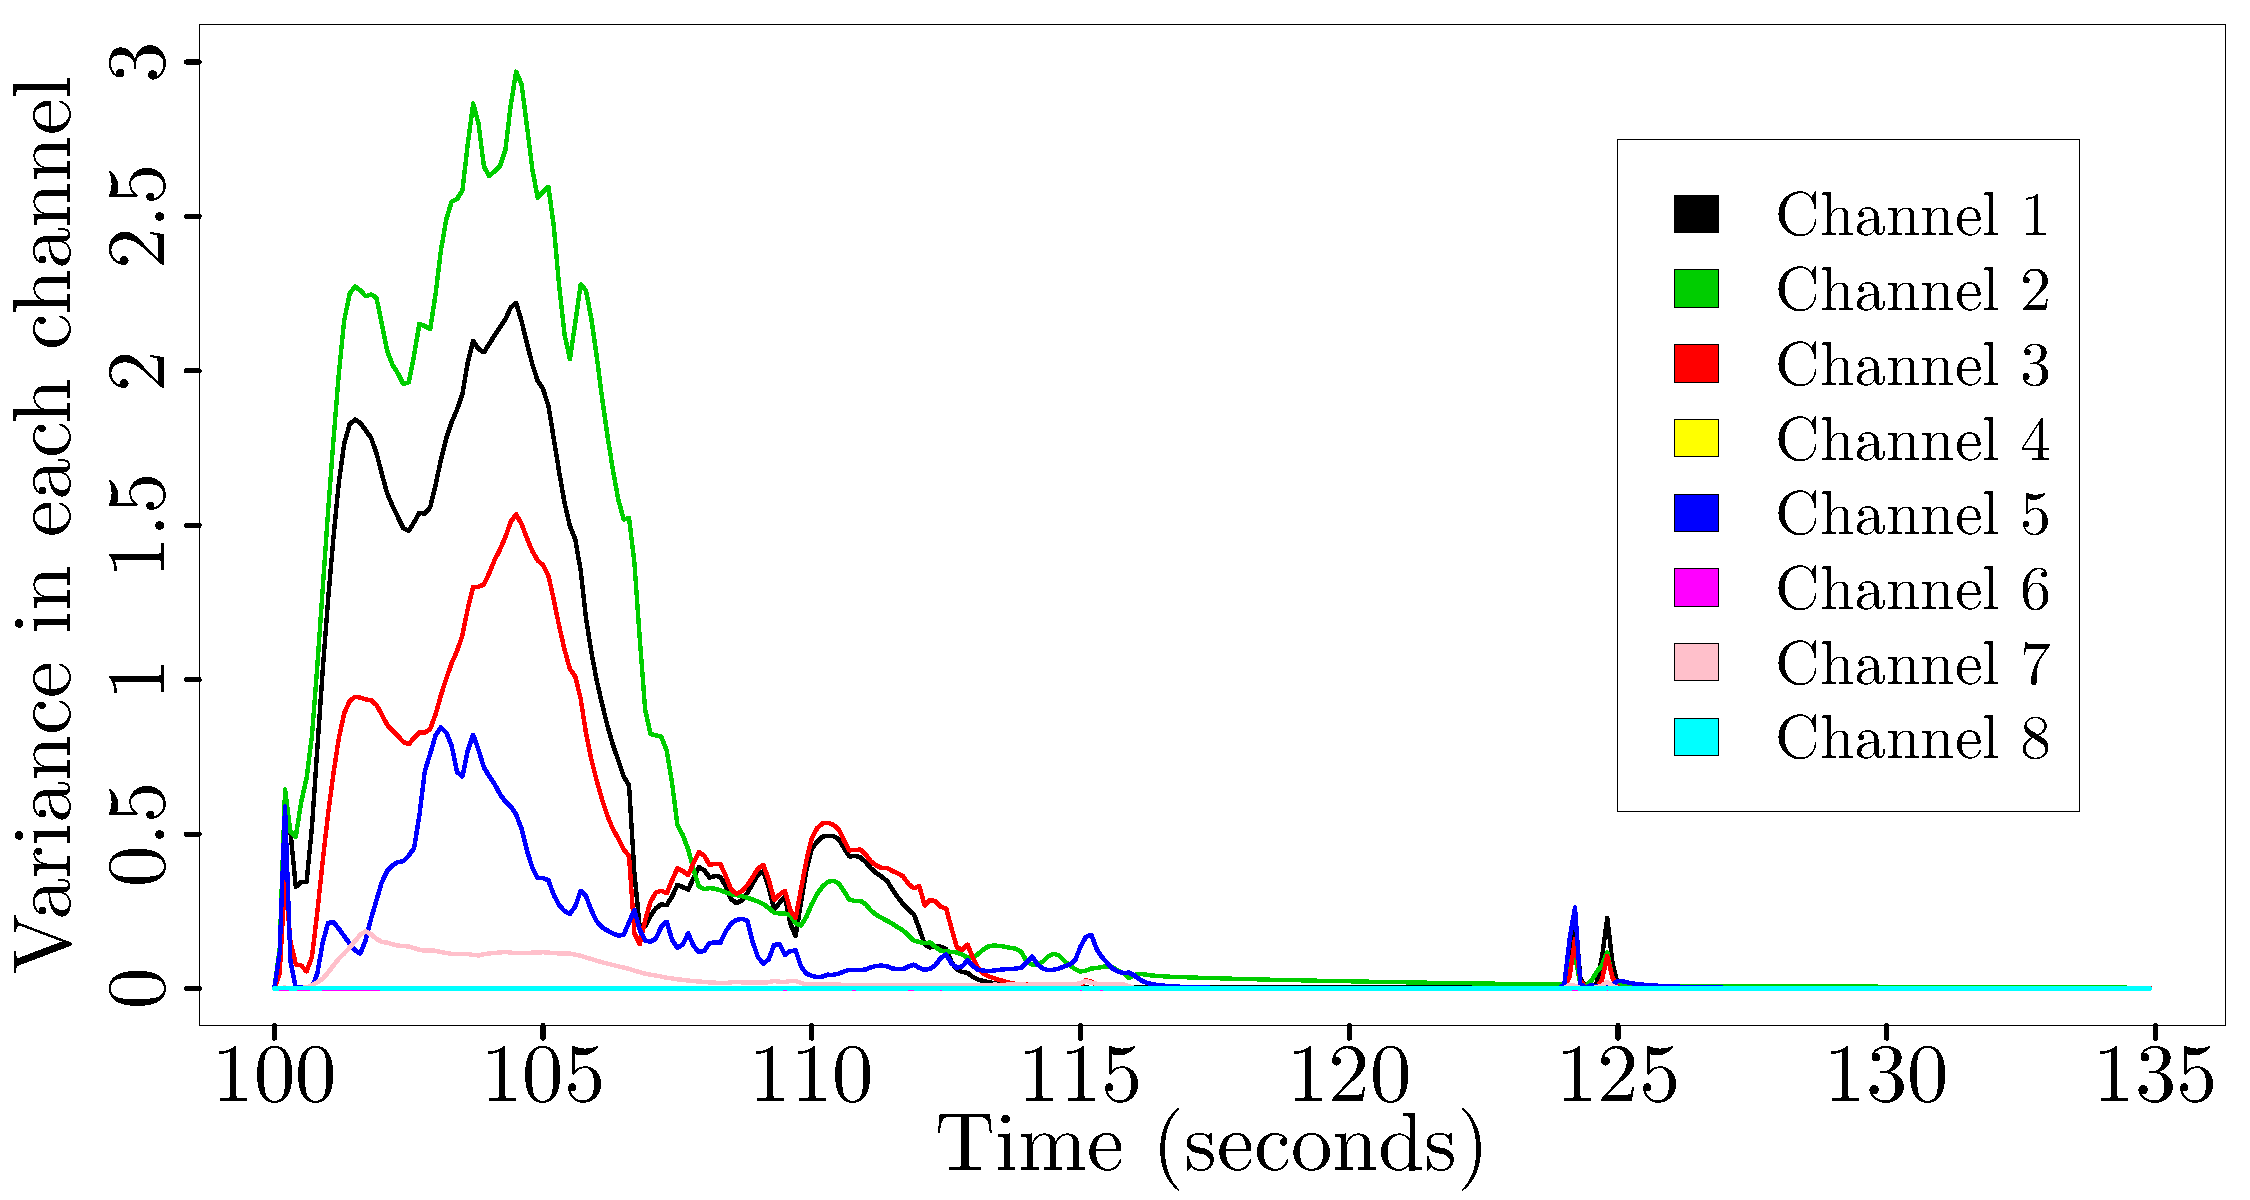
\includegraphics[scale=.25]{Figures/Channel_Variance_Comparison.pdf}
\end{center}
\caption{Variance of the $K_e$ profile when varying parameters within each channel and fixing others to their nominal values.}
\label{fig:channelwise_variances}
\end{figure}

\newpage

\begin{figure}[h]
\begin{center}
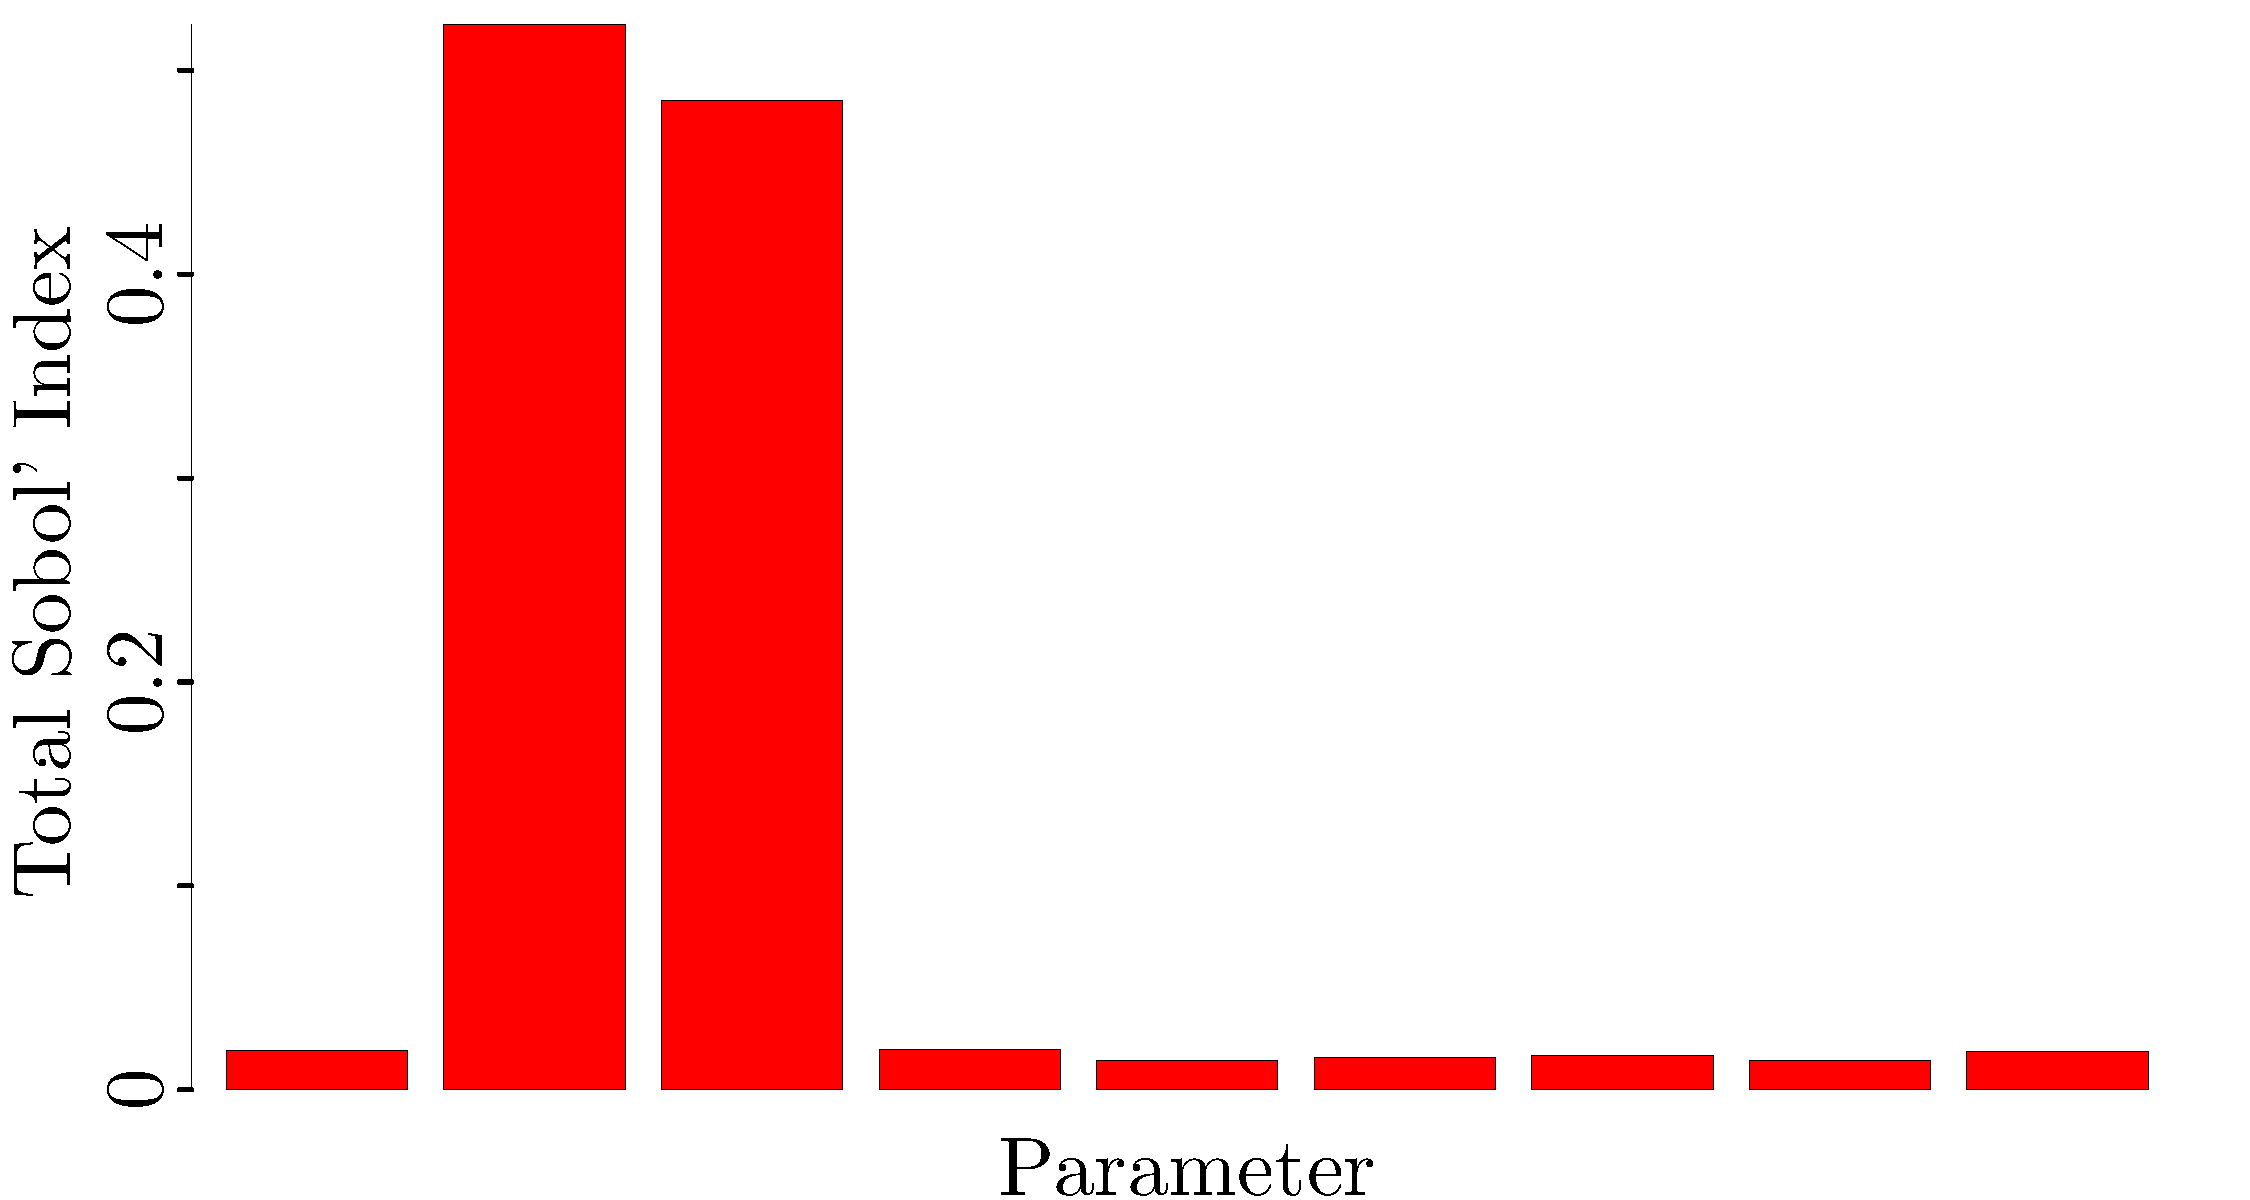
\includegraphics[scale=.2]{Figures/Channel_1_Parameters.pdf}
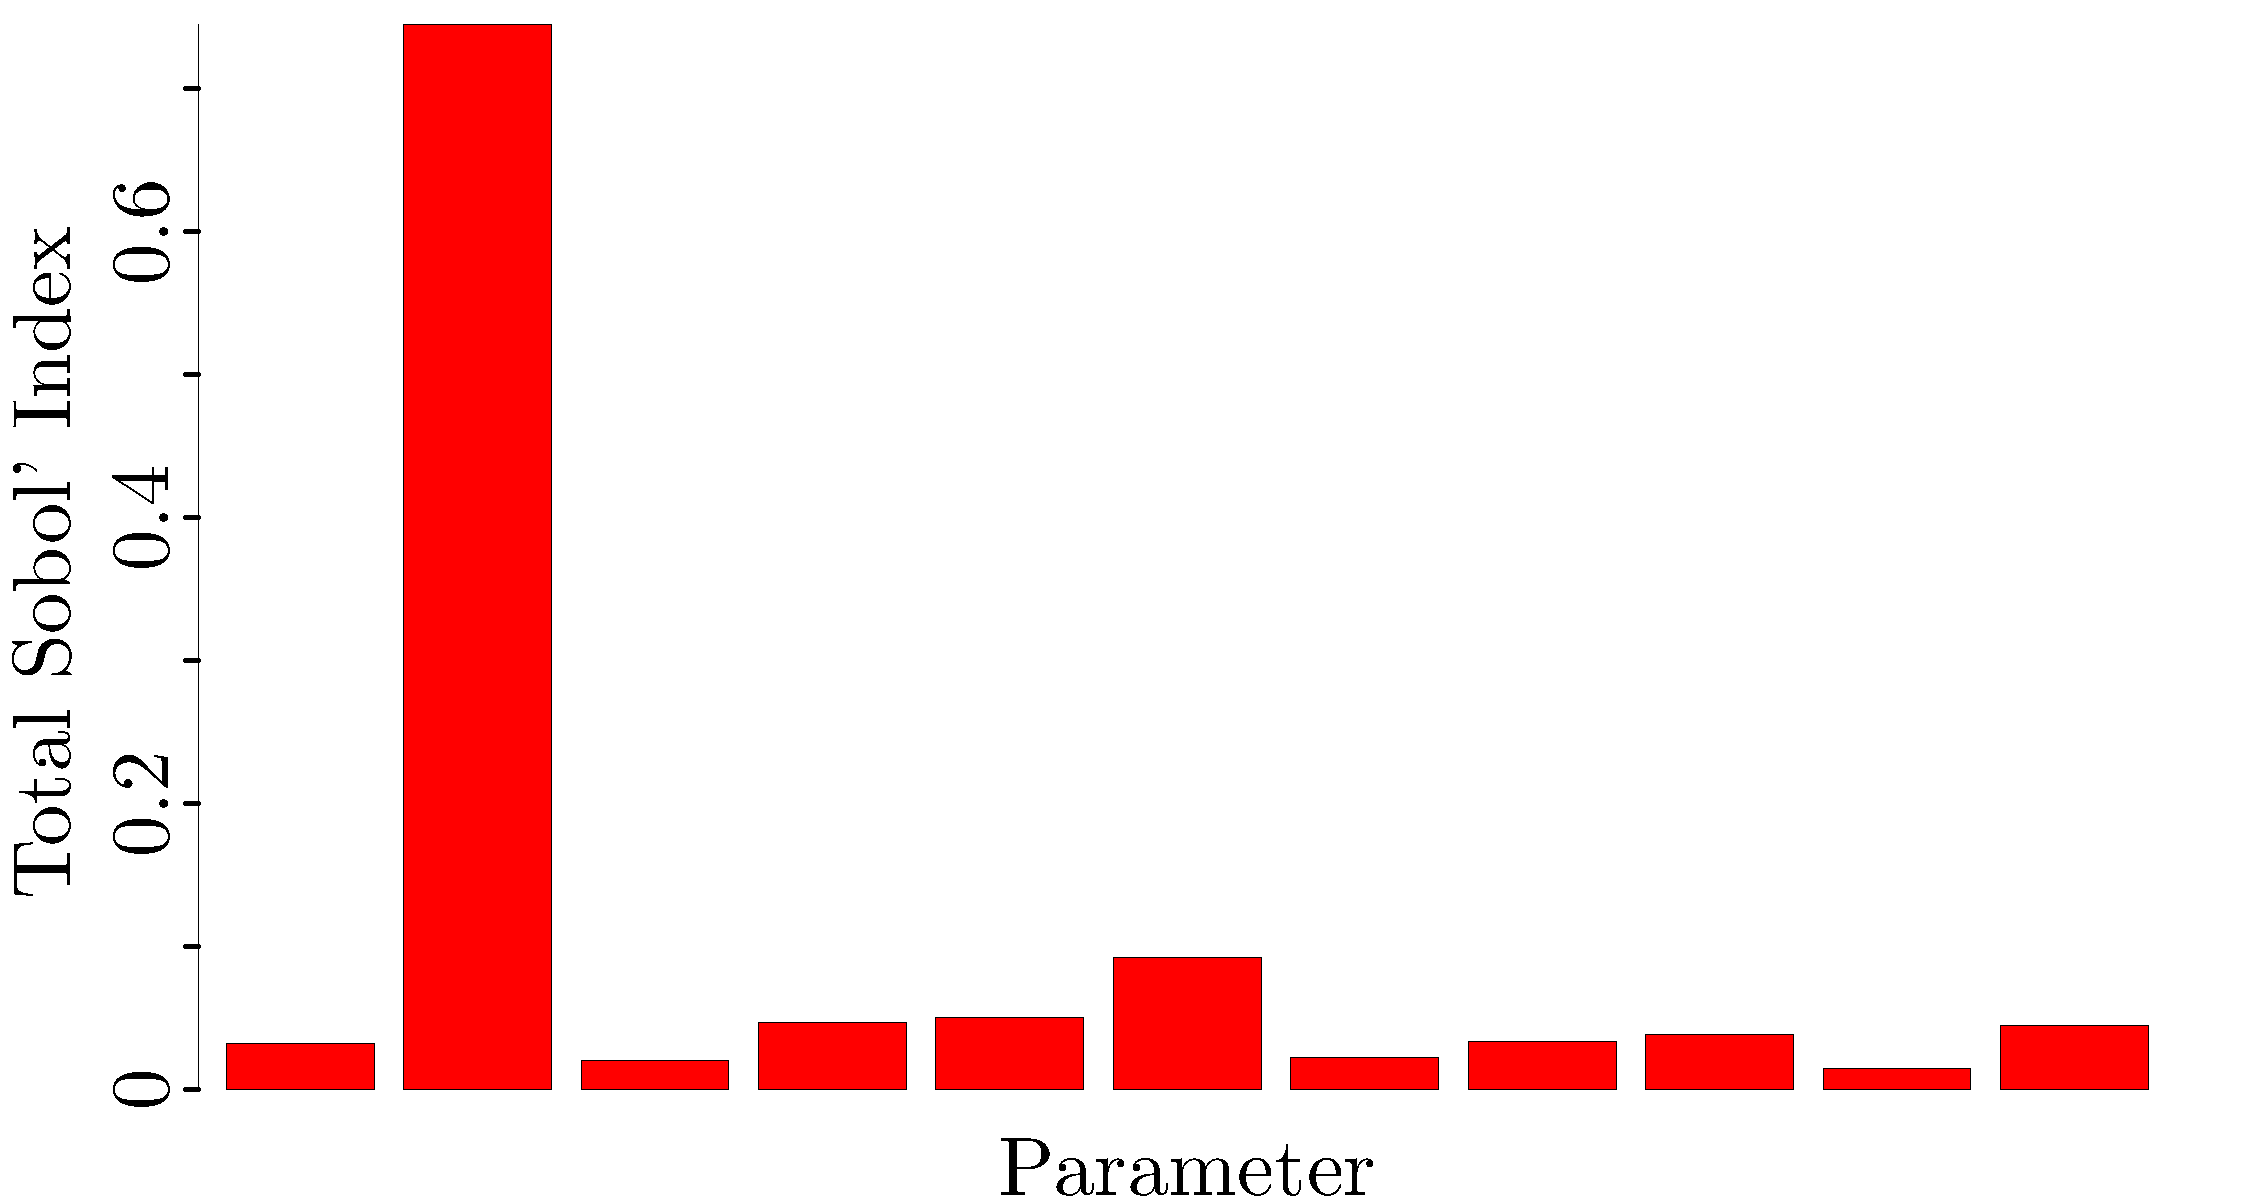
\includegraphics[scale=.2]{Figures/Channel_2_Parameters.pdf}
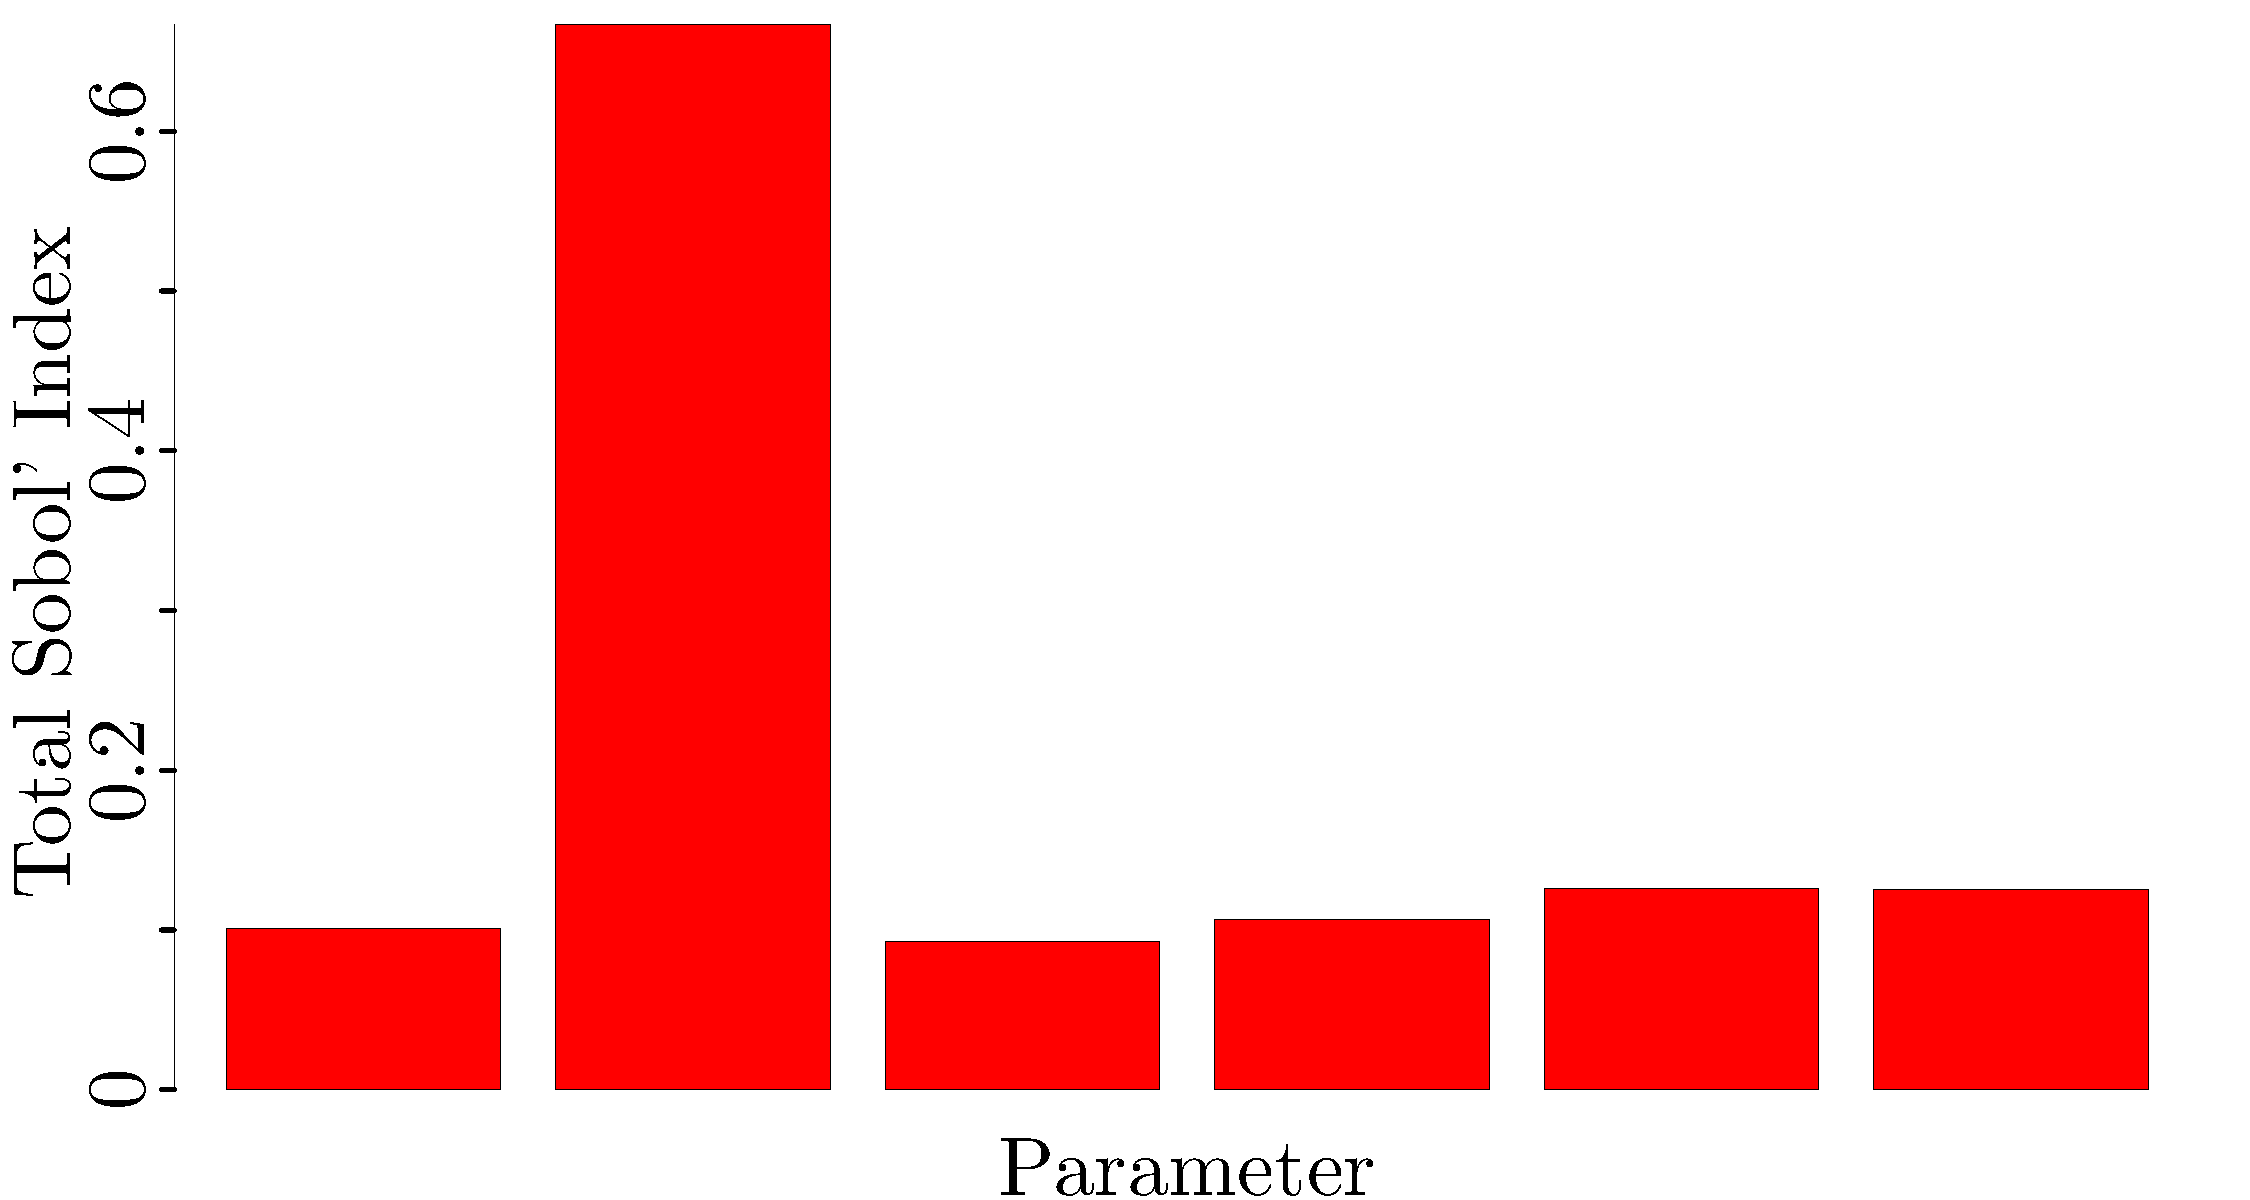
\includegraphics[scale=.2]{Figures/Channel_3_Parameters.pdf}
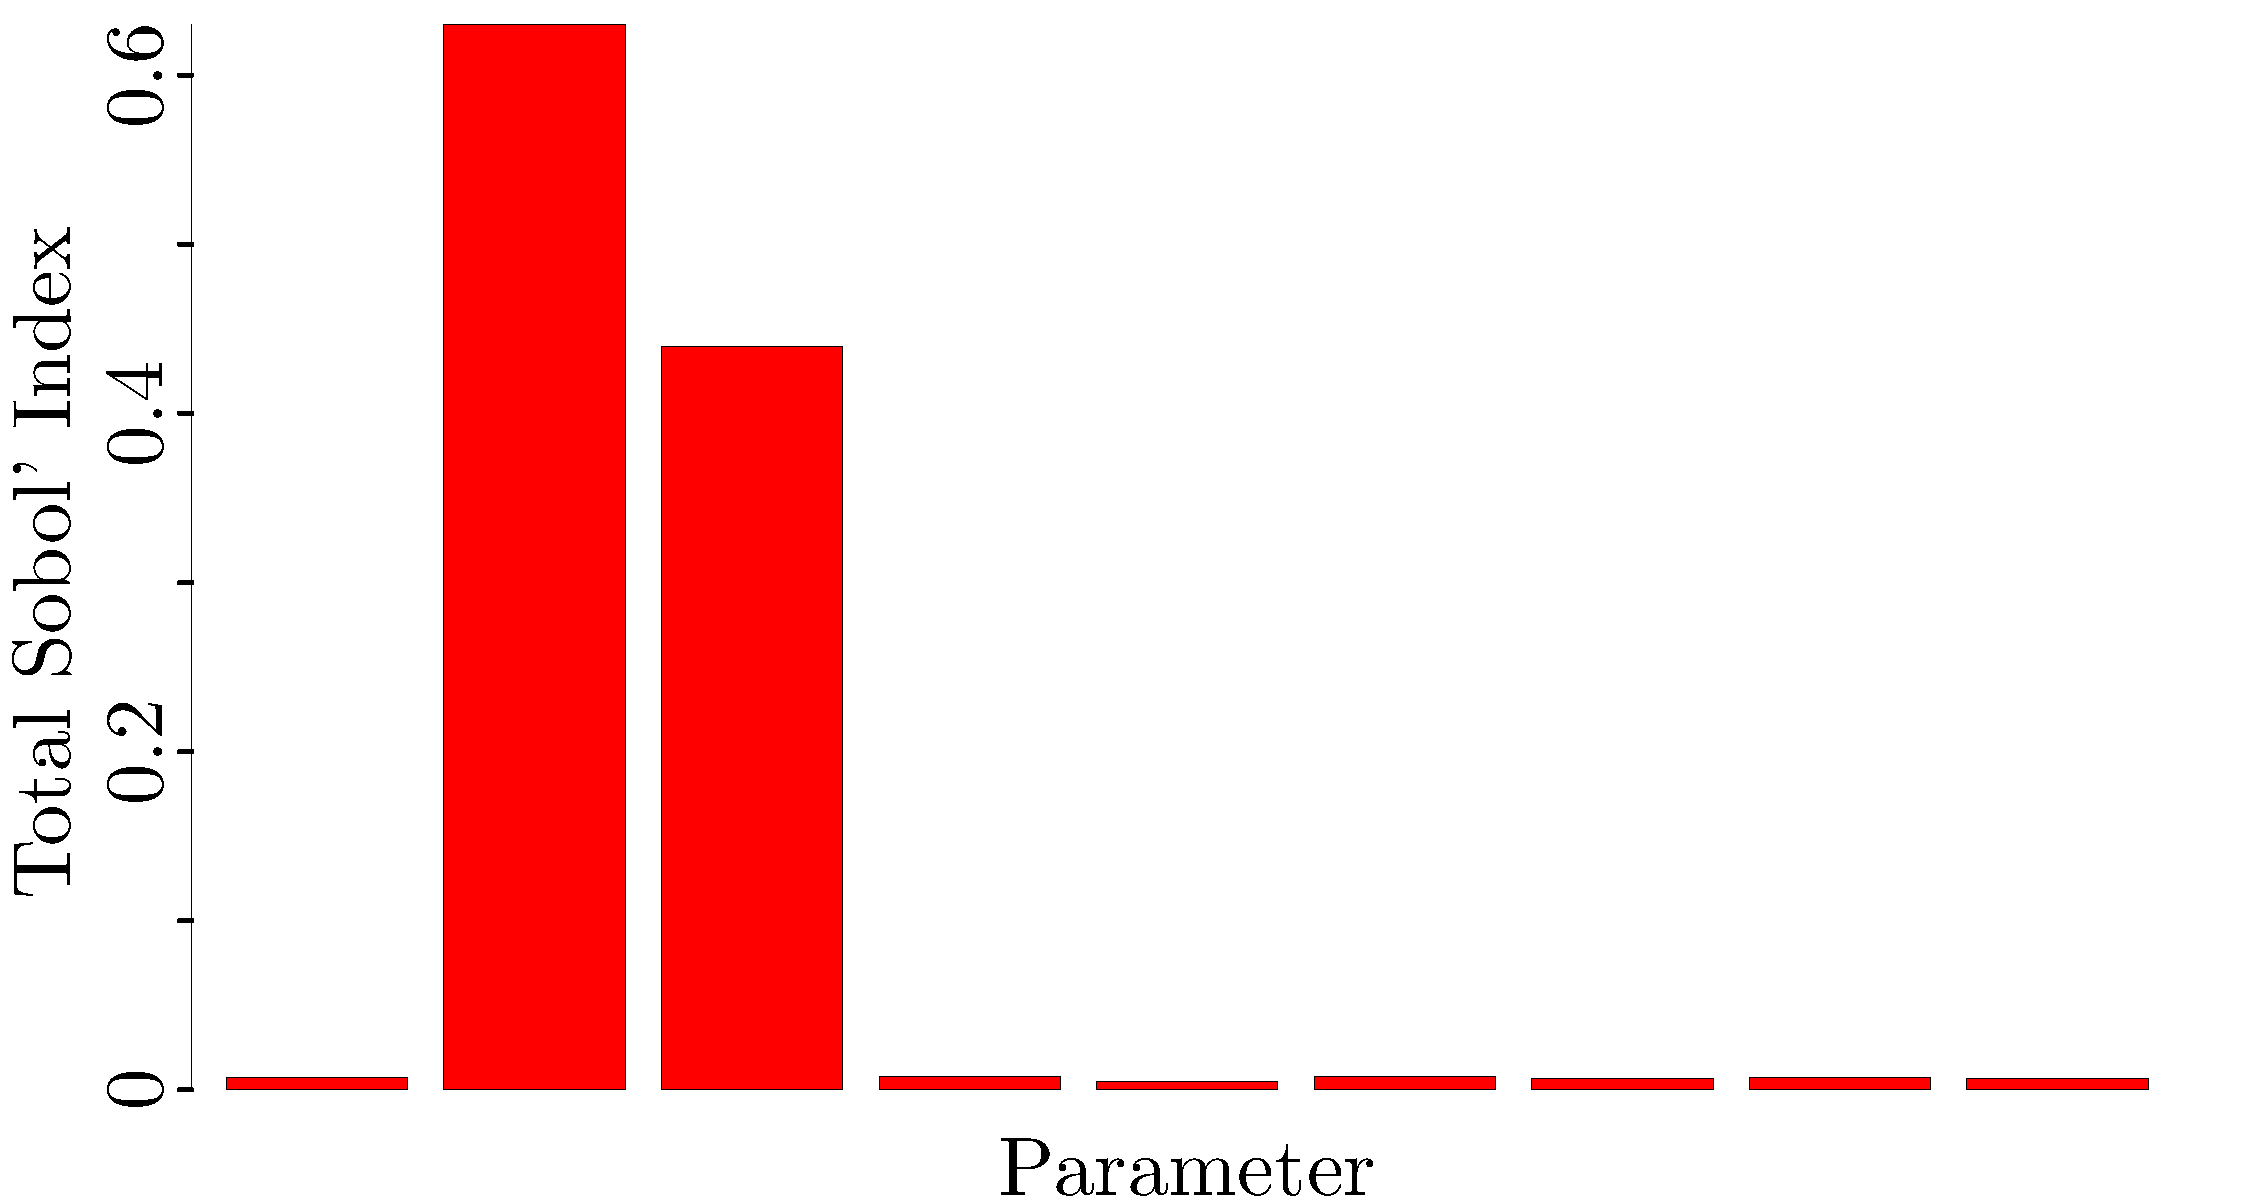
\includegraphics[scale=.2]{Figures/Channel_5_Parameters.pdf}
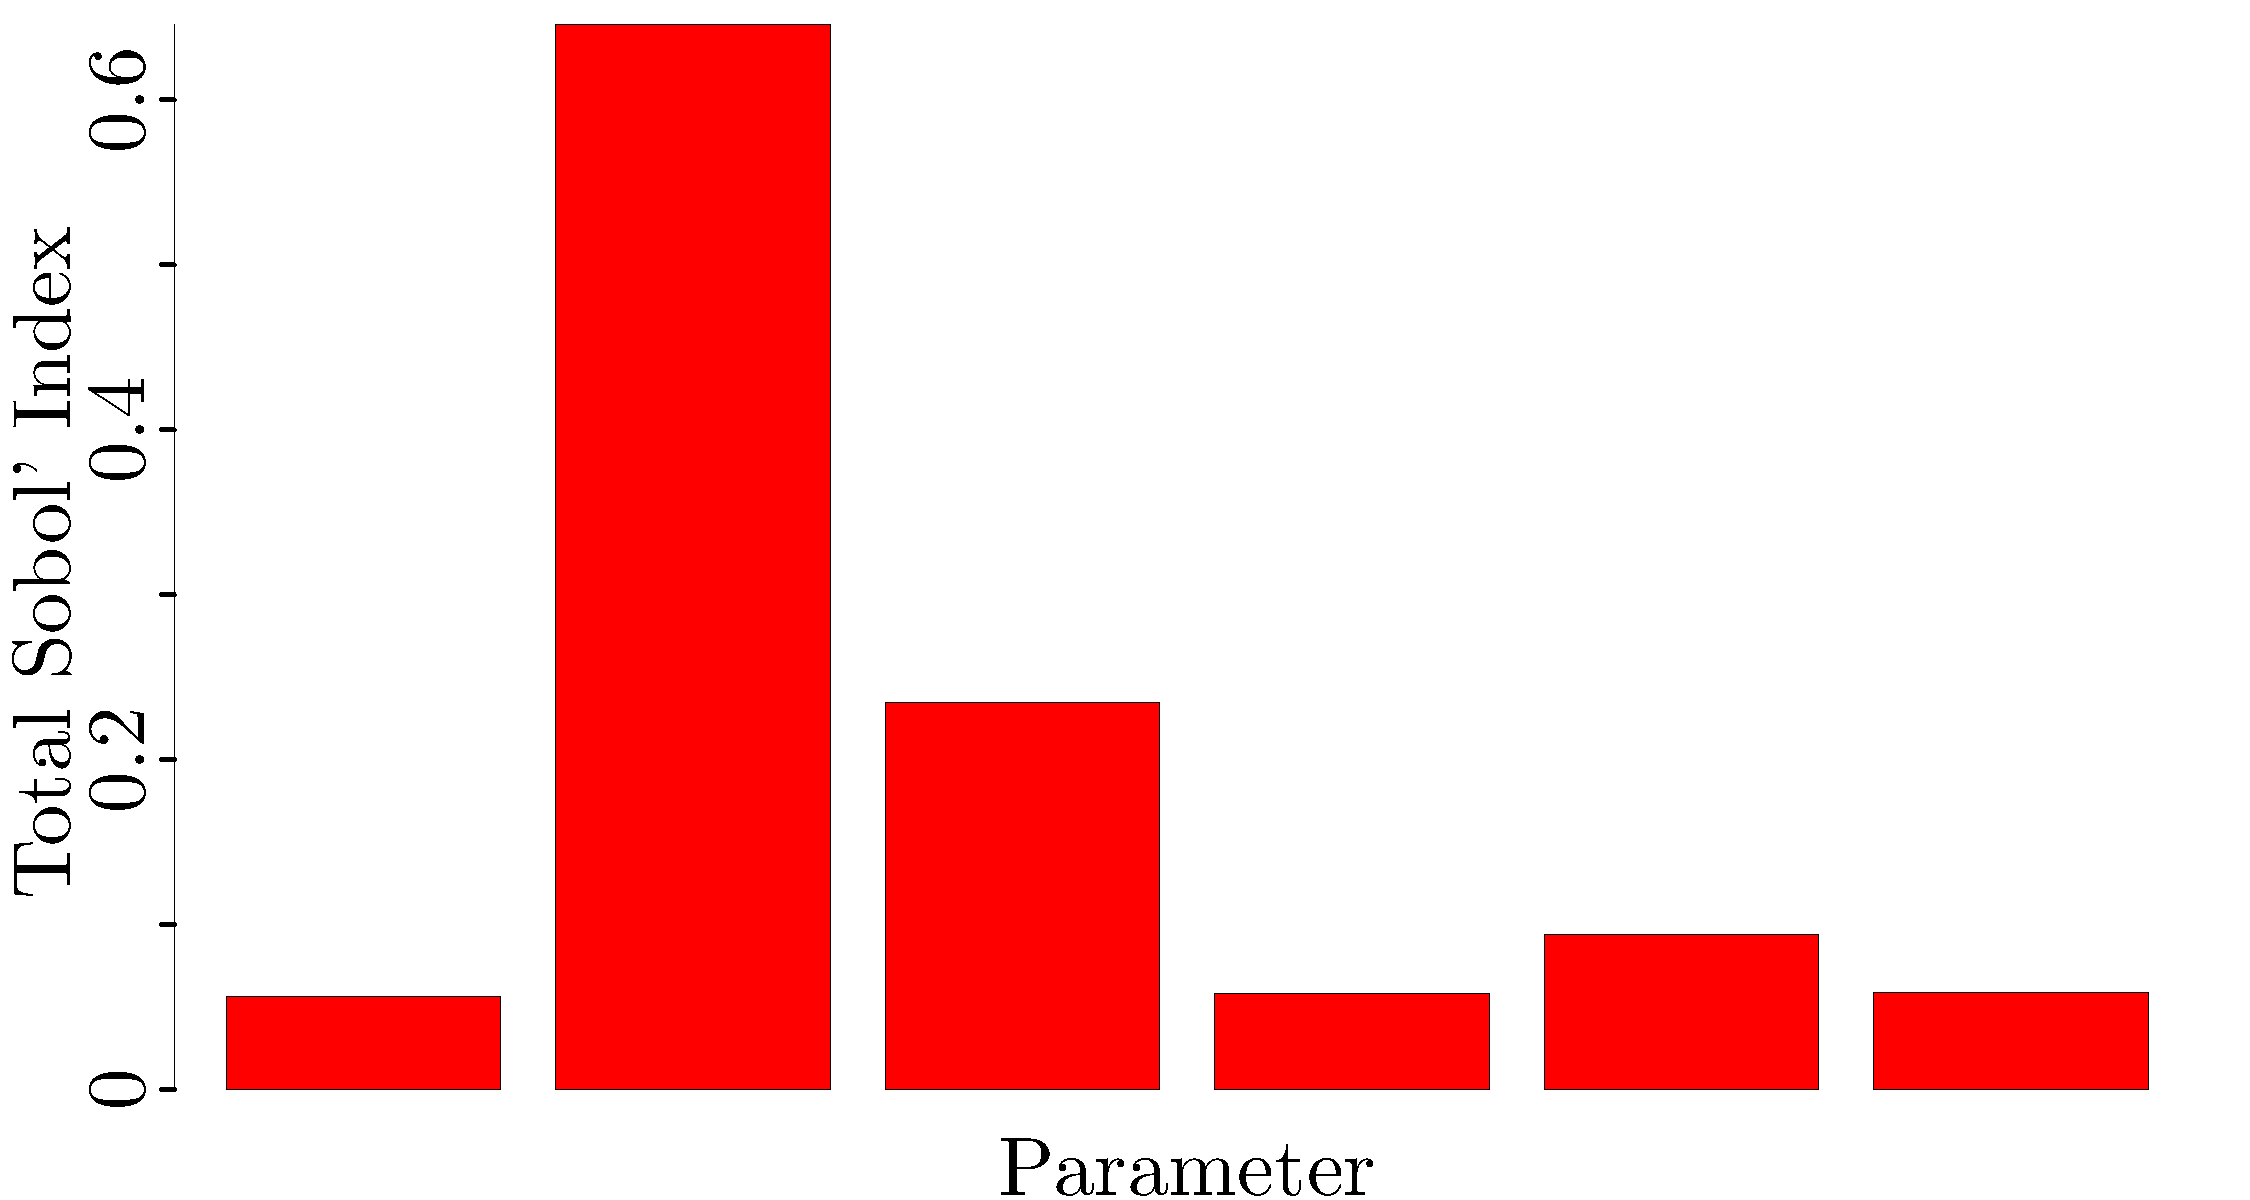
\includegraphics[scale=.2]{Figures/Channel_7_Parameters.pdf}
\end{center}
\caption{Total Sobol' indices for parameters in channels 1,2,3,5, and 7. Channel 1 is in the top left, channel 2 the top right, channel 3 the middle left, channel 5 the middle right, and channel 7 at the bottom. In each case all other parameters are fixed to their nominal values so these results ignore interactions of parameters across channels.}
\label{fig:channelwise_sobol}
\end{figure}


\newpage

Using the results of Figure~\ref{fig:all_parameters} we deduce that only 13 of the original 70 parameters should be varied. We also suspect that the NO pathway is influential so we perform a similar analysis on its parameters. There are 58 parameters which we vary, they are described in the document Tim wrote, "uncertainty\_quantification/Working\_Documents/Code\_Description/NO\_Pathway\_version\_2.pdf." We computed 1000 realizations and constructed a surrogate model using the KL expansion with radial basis functions. The Sobol' indices were computed using the surrogate model, they are shown in Figure~\ref{fig:NO_pathway_all_parameters}.

\begin{figure}[h]
\begin{center}
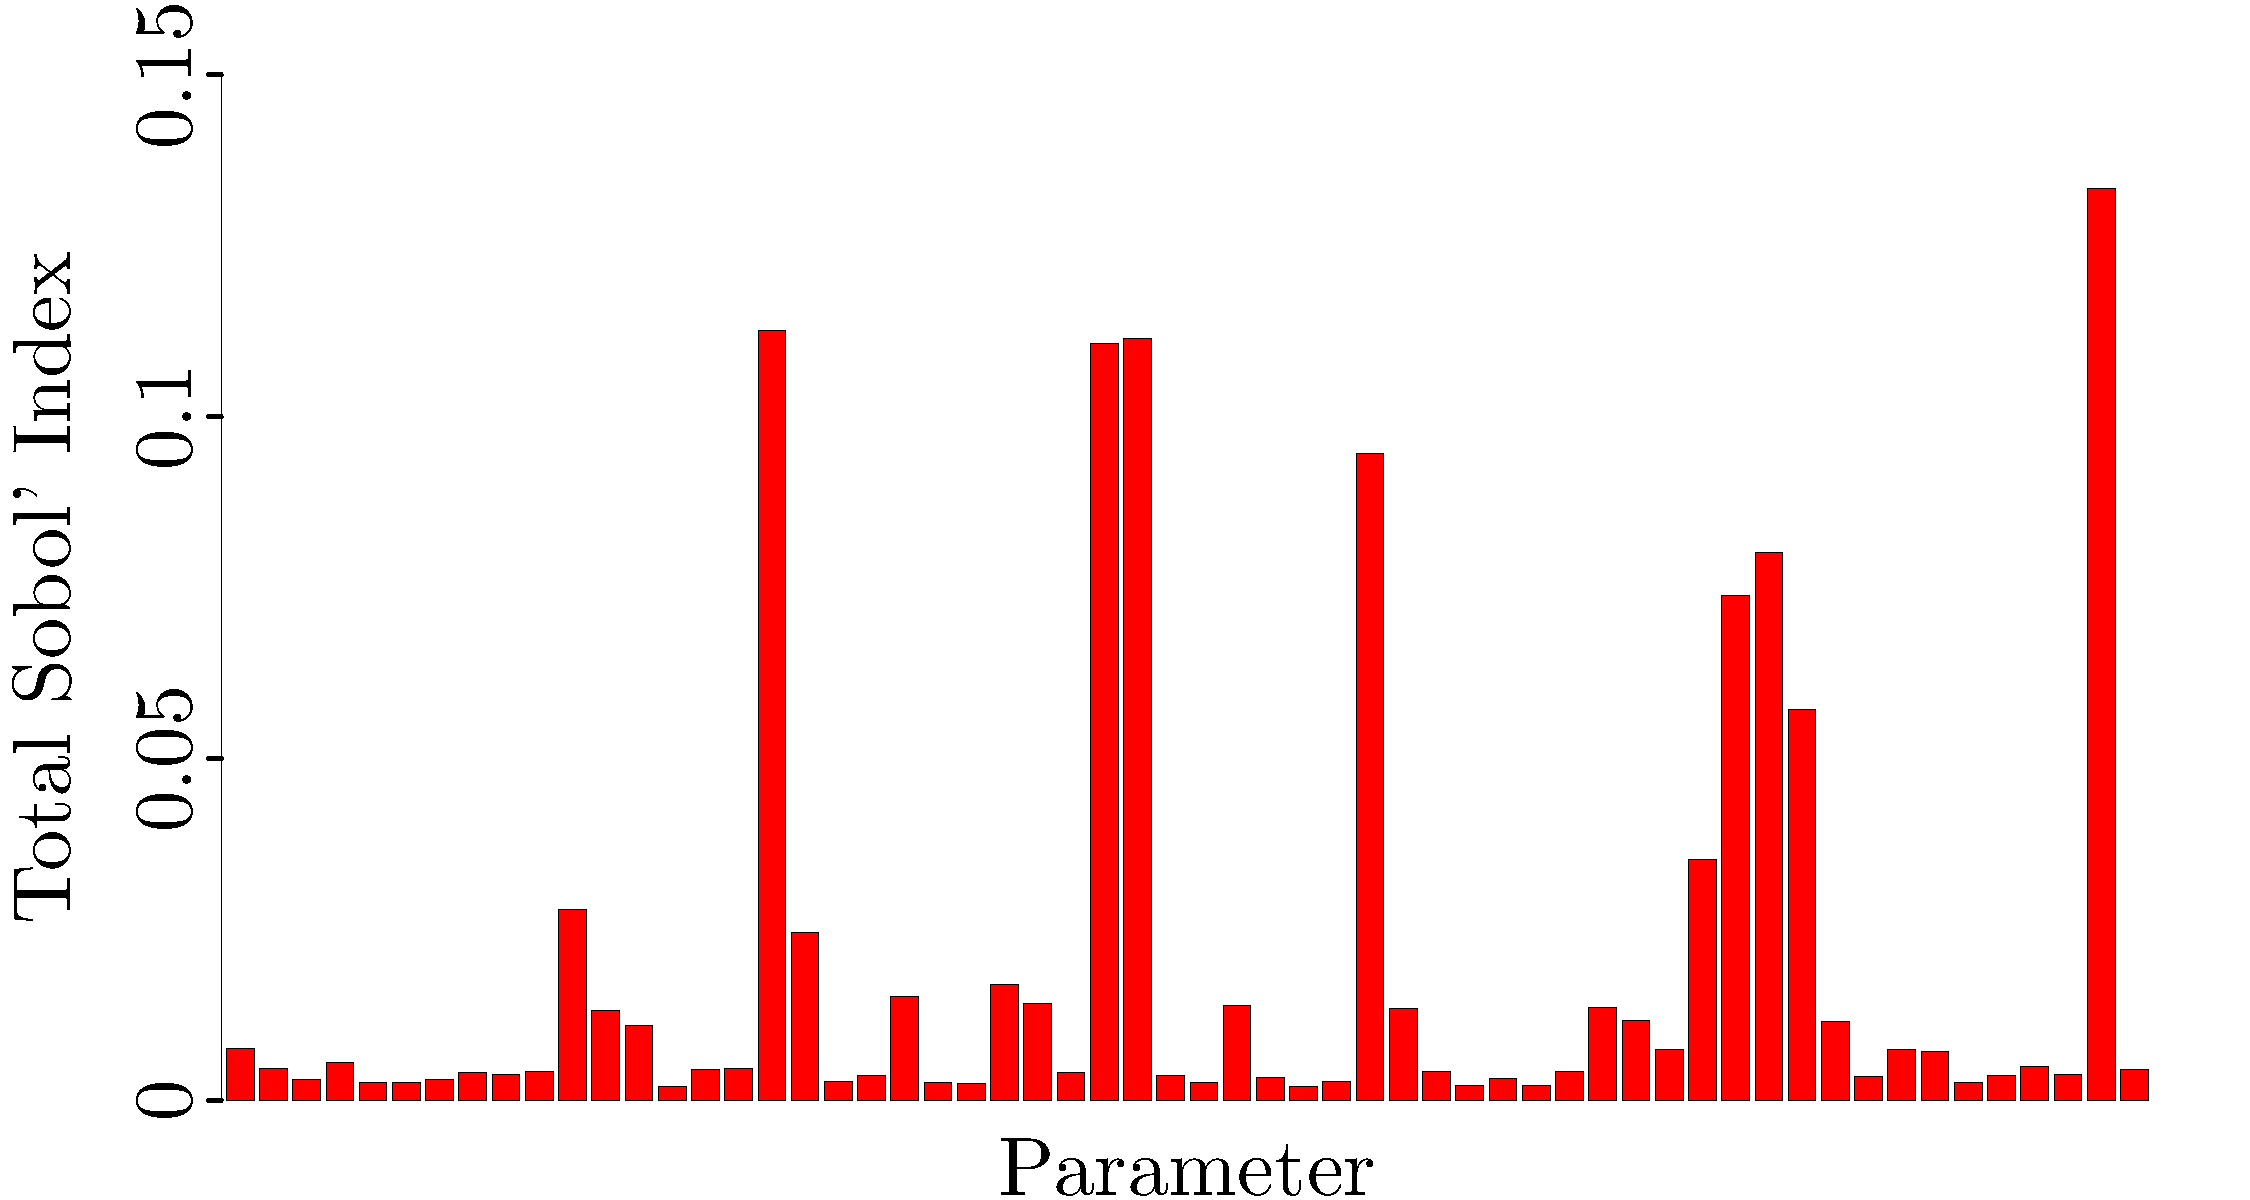
\includegraphics[scale=.25]{Figures/NO_Pathway_All_Parameters.pdf}
\end{center}
\caption{Total Sobol' indices for 58 NO pathway parameters. There are 11 parameters whose total Sobol' index is greater than 0.02 and 21 parameters whose total Sobol' index is greater than 0.01.}
\label{fig:NO_pathway_all_parameters}
\end{figure}

The 11 most influential parameters, in order, are
\begin{enumerate}
\item ('$x_{ki}$', 25);  [um];  (M.E.) in SMCEC
\item ('$x_{nk}'$, 25);             [um] ;  (M.E.) in Neuron
\item ('$x_{ki}$', 25);             [um] ;  (M.E.) in Astrocyte
\item ('$x_{nk}$', 25);             [um] ;  (M.E.) in Astrocyte
\item  ('$K_{m_{mlcp}}$', 5.5);  [uM] ; in SMCEC
\item ('$k_{pde}$', 0.0195);  [$s^{-1}$] ; in SMCEC
\item  ('$V_{max_{sGC}}$', 0.8520);  [] ; in SMCEC
\item ('$C_4$', 0.011);  [$s^{-1} microM^{-2}$]  in SMCEC
\item ('k3', 3);  [$uM^{-1} s^{-1}$] ; in SMCEC
\item ('$V_{max_{NO_{n}}}$', 4.22);     [$s^-1$] ; maximum catalytic rate of NO production (Chen2006) - obtained from fig 6 and equ 17 and 18 in Neuron
\item ('$D_{cNO}$', 3300);          [$um^2 s^-1$] ; Diffusion coefficient NO (Malinski1993) in Neuron
\end{enumerate}

\commTim{Tim may insert a comment like this.}
\commJoey{Joey may insert a comment like this.}

This is a test.

\end{document}